The system is designed to be as modular as possible, allowing for testing and implementation of a number of different algorithms and processing steps without having to spend a lot of time integrating these with the rest of the system. Tuning without having to re-compile the project was also a major goal that was achieved by using a set of configuration files that specify parameter values at startup.


\begin{figure}[htb]
	\centering
	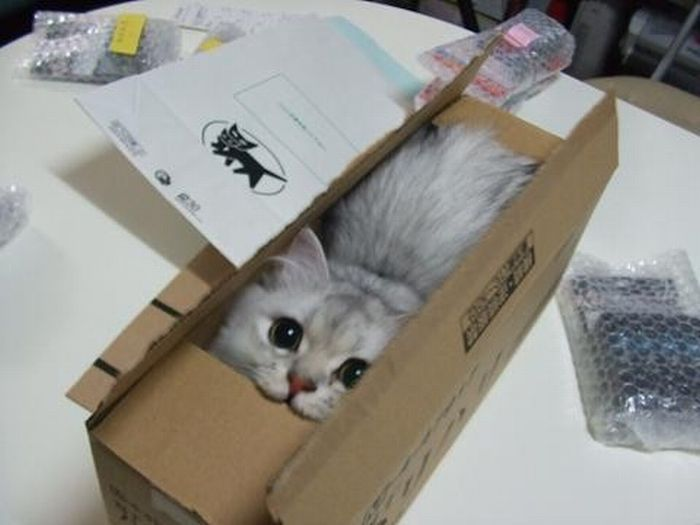
\includegraphics[width=\linewidth]{images/boxcat.jpg}
	\caption[Overview of the entire system]{\textit{System overview.}}
	\label{fig:system_overview}  %Skapar referens till figuren
\end{figure}

\subsection{Configuration file system}
The system configuration file contains all image processing pipeline parameters, including which image processing algorithms to run and in what order. together with the address of the current destination web service, where counting results are to be presented. There is also a GUI configuration file containing the Debug GUI as well as camera specific settings. 

\subsection{Network module}
The network module manages all system input/output, i.e. sampling the sensors and posting output data on the web server specified by the configuration file. Currently, support exists for all OpenCV-compatible cameras as well as the Microsoft Kinect depth sensor. The module is designed to be as modular as possible, allowing for a relatively easy integration of new sensor types into the system. The network module also supports running several sensors in parallel. 

\subsection{Algorithm Interface}
The algorithm interface simplifies the addition of new image processing or tracking modules to the system. Together with the config file, this allows a very flexible software system that could be used for virtually any computer vision problem. (Add more here)

\subsection{Debug and Config GUI}
Debug GUI features (Image and stuff)
Configuration GUI management (more image and such)
